\documentclass[11pt]{article}
\usepackage[margin=1in]{geometry}
\usepackage{amsmath,amssymb}
\usepackage{graphicx}
\usepackage{booktabs}
\usepackage{xcolor}
\usepackage[numbers,sort&compress]{natbib}
\usepackage[hidelinks]{hyperref}
\usepackage{microtype}

\newcommand{\todo}[1]{\textcolor{red}{[TODO: #1]}}
% every number quoted from experiments: generated by scripts/make_paper_numbers.py
% generated by scripts/make_paper_numbers.py
\newcommand{\GEOsizeOvTen}{0.05}
\newcommand{\GEOsizeOvHundred}{0.49}
\newcommand{\GEOsizeFourKTen}{0.14}
\newcommand{\GEOsizeBcTen}{0.02}
\newcommand{\GEOparOvCornerTen}{1.8}
\newcommand{\GEOparBcTen}{3.4}
\newcommand{\GEOshOvTen}{3.8}
\newcommand{\GEOshBcTen}{5.0}
\newcommand{\NumShots}{200}
\newcommand{\NumTrain}{140}
\newcommand{\NumTest}{60}
\newcommand{\NumTestFrames}{7{,}403}
\newcommand{\PosFrac}{10.0}
\newcommand{\NumEvents}{39}
\newcommand{\TRKmedianOverhead}{0.26}
\newcommand{\TRKninetyOverhead}{336.60}
\newcommand{\TRKmedianBroadcast}{0.29}
\newcommand{\TRKninetyBroadcast}{65.86}
\newcommand{\TRKcentreErr}{0.29}
\newcommand{\INPUTCLIPROWS}{\texttt{break} & Full-rack break with a slightly elevated cue: cue ball and object balls hop off the cloth briefly. & 9\,mm \\
\texttt{elevated\_draw} & Draw shot with an elevated cue (14 deg). Borderline: a $\sim$1 cm hop. & 9\,mm \\
\texttt{jump\_clips\_blocker} & Jump too low: cue ball strikes the top of the blocker, which hops. Positive, with a secondary object-ball hop. & 75\,mm \\
\texttt{jump\_over\_blocker} & Cue ball jumps a blocker 28 cm away and hits the 1-ball. Positive. & 101\,mm \\
\texttt{long\_jump\_off\_axis} & Long, fast jump along the side rail, far from the overhead camera's optical axis (large parallax). Positive. & 89\,mm \\
\texttt{near\_miss} & Cue ball passes 4 mm beside a ball without leaving the cloth: in 2-D the two balls almost touch. Hard negative. & 1\,mm \\
\texttt{stop\_shot} & Level stun shot, cue ball stops dead. Negative. & 0\,mm \\}


\title{Did It Leave the Cloth?\\Detecting Airborne Balls in Pool Video from Overhead and Broadcast Cameras}
\author{Working draft --- billiard-research}
\date{\today}

\begin{document}
\maketitle

\begin{abstract}
Jump shots, hops off the break and balls that ride up over one another are
routine in pool, but every vision system for the game we know of treats the
balls as points on a plane. We ask how well a fixed camera can tell when a
ball has left the cloth, and which visual evidence carries that information.
Because no billiards dataset labels ball height, we build one: a 3D billiards
simulator with an airborne phase (ballistic flight, slate bounces, 3D
ball--ball collisions) coupled to a physically based renderer that produces
video from an overhead table camera and from an elevated broadcast camera,
with exact per-frame height ground truth. A geometric analysis shows that the
cue most often proposed for overhead cameras, apparent ball size, is
essentially unusable: a ball 1\,cm off the cloth grows by
\GEOsizeOvTen\,px at 720p (\GEOsizeFourKTen\,px at 4K), while the shadows cast by off-axis lamps
move by several pixels per centimetre. We then evaluate a detector built on three
pixel-derived cue families --- size, shadow and motion (a rolling-versus-ballistic
model comparison) --- on \NumTest{} held-out randomised shots.
\INPUTRESULTABSTRACT
We release the simulator, renderer, clips and detector, and describe a
protocol for collecting real clips with height ground truth.
\end{abstract}

\section{Introduction}

Computer vision for cue sports has largely been about finding balls on a
plane: detect each ball in each frame, map it to table coordinates and track
it~\citep{roboflow2023pool}. That plane assumption breaks during some of the
game's most consequential moments. A jump shot deliberately drives the cue
ball into the slate so it rebounds over an obstructing ball; a hard break
often lifts the cue ball and object balls off the cloth; and a jumped ball that
clips the top of another ball can send either one airborne. Whether a ball
left the cloth matters for rules (an illegal ``scoop'' under the ball versus a
legal jump), for shot analytics and coaching, and for any system that
reconstructs or simulates the game: a tracker that assumes planar motion
silently misplaces an airborne ball and misreads apparent collisions.

This raises a simple question with no published answer: \emph{from a
single fixed camera, how reliably can we detect that a ball is airborne,
and which visual evidence makes it possible?} The two camera placements that
dominate practice behave very differently. An overhead table camera, the
standard choice for streaming and analytics rigs, looks along the very axis
in which the ball moves. An elevated broadcast camera behind the end rail
sees height directly but foreshortens the table.

\paragraph{Contributions.}
\begin{enumerate}
  \item A billiards simulator with an airborne phase and a renderer that turns
        its output into video from both camera placements with exact per-frame
        height labels (Sec.~\ref{sec:sim}). Existing open simulators keep every
        ball on the table~\citep{kiefl2024pooltool}.
  \item A geometric analysis of the information each cue carries per
        millimetre of height, per camera and per image resolution
        (Sec.~\ref{sec:geometry}). It predicts which cues can work before any
        learning is involved.
  \item A transparent detector built on pixel-level size, shadow and motion cues,
        evaluated per cue family and per camera, including both views fused
        (Secs.~\ref{sec:detector}--\ref{sec:results}).
  \item Seven hand-designed scenario clips that isolate the situations a
        detector must handle (Table~\ref{tab:clips}), and a protocol for
        collecting real clips with height ground truth (Sec.~\ref{sec:real}).
\end{enumerate}

\section{Related work}

\paragraph{Cue-sport vision and simulation.}
Ball detection and tracking for pool is well served by off-the-shelf object
detectors~\citep{roboflow2023pool}, and analytic physics engines simulate
shots precisely on the plane of the table~\citep{leckie2006event,kiefl2024pooltool}.
The physics of jump shots, including the role of the slate rebound, is
discussed in the billiards literature~\citep{marlow1995physics,alciatore_tpb10},
but to our knowledge no vision work detects or measures airborne balls, and
no public dataset labels ball height.

\paragraph{Monocular 3D ball trajectories in other sports.}
Recovering ball height from one camera is better studied in tennis and table tennis.
\citet{ponglertnapakorn2025where} lift 2D tennis tracks to 3D and stress that
a 2D trajectory is consistent with many 3D motions. \citet{kienzle2025spin}
train a network purely on physics-simulated trajectories and report transfer to
real table-tennis broadcasts, and \citet{kienzle2026uplifting} build a robust
two-stage pipeline for real footage. We follow the same synthetic-to-real
philosophy, but pool differs in ways that change which cues work: the ball is
small in the image, the camera is often directly above the action, flights are
short (a few to a few dozen frames), and the lighting is a fixed set of lamps
close to the table, which makes shadows unusually informative.

\section{Simulation and rendering}\label{sec:sim}

\paragraph{Physics.}
Balls are rigid spheres ($R=28.6$\,mm, $m=170$\,g) on a 9-ft table, integrated
at 2.4\,kHz. On the cloth we use the standard sliding/rolling/spinning model
(sliding friction $\mu_s=0.2$, rolling resistance $\mu_r=0.01$). Off the
cloth a ball follows a ballistic path; air drag is negligible over sub-second
flights. A landing applies a normal impulse with restitution $e_t=0.5$ and a
Coulomb friction impulse at the contact point; rebounds slower than
0.04\,m/s end the bounce sequence. Ball--ball collisions are resolved in 3D,
so a high enough ball clears a blocker, and a low one strikes its upper hemisphere,
driving it into the slate and making it hop. A jump shot is modelled the way it
happens physically: the cue sends the ball \emph{down} into the slate at the
cue elevation, and the first landing impulse turns that into the jump.
Cushions are walls of height 45\,mm, and pockets swallow balls whose centres
enter them. Table~\ref{tab:params} lists the parameters; $e_t$ is a little below
the typical 0.6 quoted by~\citet{alciatore_tpb10}, and checking sensitivity to it is
future work.

\paragraph{Rendering.}
A ray caster renders the table (cloth, cushions, rails, pockets) and the
balls (solid and striped textures with number discs, rotating with the
simulated angular velocity, glossy highlights). The room has three hanging lamps,
each an area light, that cast soft shadows on the cloth and on other balls.
Each pixel takes four samples jittered within the pixel and within the shutter
interval, which gives anti-aliasing and physically correct motion blur. Frames are
tone-mapped, get Gaussian sensor noise, and are H.264-encoded at 60\,fps. Two
calibrated cameras are rendered: \textbf{overhead}, looking straight down from
2.6\,m, and \textbf{broadcast}, behind the foot rail at a height of 1.55\,m
(Fig.~\ref{fig:frames}). Both are 1280$\times$720. For each clip we also store
the empty-table frame a fixed camera can capture once.

\paragraph{Ground truth.}
For every frame and ball we store the centre at mid-exposure, the maximum
height of the ball's lowest point above the cloth during the exposure, and
whether that exceeds 1\,mm.

\begin{table}[t]
\centering\small
\begin{tabular}{llll}
\toprule
Parameter & Value & Parameter & Value \\
\midrule
Ball radius / mass & 28.575\,mm / 170\,g & Ball--ball restitution & 0.95 \\
Sliding / rolling friction & 0.2 / 0.01 & Ball--slate restitution $e_t$ & 0.5 \\
Landing friction & 0.2 & Cushion restitution & 0.8 \\
Integration rate & 2400\,Hz & Video & 60\,fps, H.264 \\
Lamps & 3 area lights, 0.95\,m up & Overhead camera & 2.6\,m, $f\!\approx\!1090$\,px \\
\bottomrule
\end{tabular}
\caption{Default simulation and rendering parameters. The randomised set
varies camera placement, lamp height and spacing, sensor noise, shutter and
exposure (Sec.~\ref{sec:protocol}).}
\label{tab:params}
\end{table}

\begin{figure}[t]
\centering
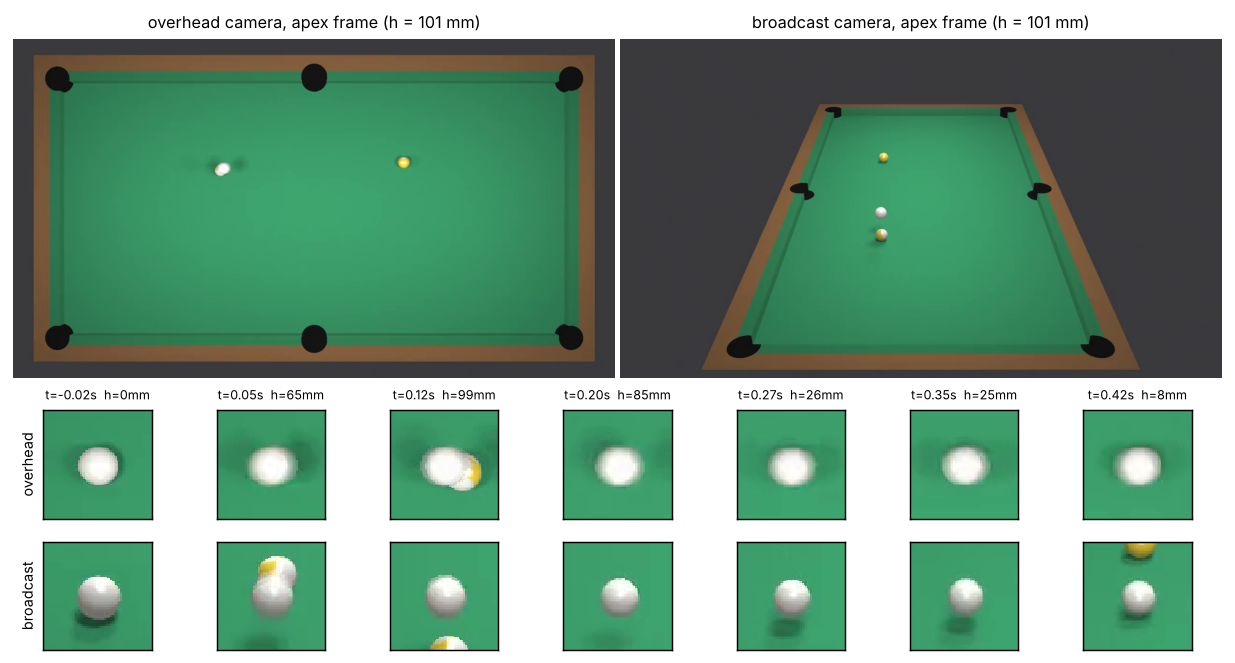
\includegraphics[width=\linewidth]{figures/frames_jump_over_blocker.png}
\caption{The \texttt{jump\_over\_blocker} clip at the apex of the jump, from the
overhead (left) and broadcast (right) cameras, with zoomed crops across the
flight. From overhead the airborne cue ball overlaps the blocker and its lamp shadows
pull away from it; from the broadcast view the ball visibly separates from its
shadow.}
\label{fig:frames}
\end{figure}

\paragraph{Scenario clips.}
Table~\ref{tab:clips} lists the seven hand-designed clips. Each isolates one
situation: clean positives, a hard negative where two balls almost touch in
the image without either leaving the cloth, a borderline centimetre hop, a
secondary object-ball hop, and the 16-ball break.

\begin{table}[t]
\centering\small
\begin{tabular}{p{3.3cm}p{9.6cm}r}
\toprule
Clip & What it tests & Cue apex \\
\midrule
\INPUTCLIPROWS
\bottomrule
\end{tabular}
\caption{The scenario clips (both camera views each). Apex is the cue ball's
maximum height above the cloth.}
\label{tab:clips}
\end{table}

\section{How much signal does each cue carry?}\label{sec:geometry}

Before learning anything, we ask how many pixels each cue moves per
millimetre of height, using the calibrated cameras alone
(Fig.~\ref{fig:geometry}).

\emph{Size.} Raising the ball by $h$ brings it closer to an overhead camera
at height $H$, scaling its image radius by $(H-R)/(H-R-h)$. At $H=2.6$\,m and
720p that is \GEOsizeOvTen\,px at $h=10$\,mm and only \GEOsizeOvHundred\,px at
100\,mm; even 4K gives \GEOsizeFourKTen\,px per centimetre. Our blur-robust
sub-pixel radius estimator has frame-to-frame noise of roughly 0.25\,px at 720p,
so apparent size is the weakest cue by an order of magnitude. The broadcast
camera fares even worse (\GEOsizeBcTen\,px), because height moves the ball across
the line of sight rather than along it.

\emph{Parallax.} An airborne ball appears displaced from where an on-cloth
ball at the same table position would be. For the overhead camera the
displacement is radial from the camera's nadir, so it is \emph{zero} directly
below the camera and \GEOparOvCornerTen\,px per centimetre near a corner.
For the broadcast camera it is \GEOparBcTen\,px per centimetre everywhere. A
single frame cannot separate this displacement from a different table
position, but a track can, because ballistic flight and rolling produce
different image-space kinematics. That is what our motion cue tests.

\emph{Shadows.} With lamps about a metre above the cloth, a ball's shadow
from a lamp at horizontal offset $d$ moves by roughly $d\,h/(L-h)$. From the
lamp directly overhead, the shadow stays hidden under the ball, but the
neighbouring lamps' shadows move by \GEOshOvTen\,px per centimetre at the table
centre in the overhead view (\GEOshBcTen\,px in broadcast). Shadows are
therefore the strongest single-frame cue overhead, \emph{provided the room
has off-axis lamps}, as typical multi-shade fixtures do.

\begin{figure}[t]
\centering
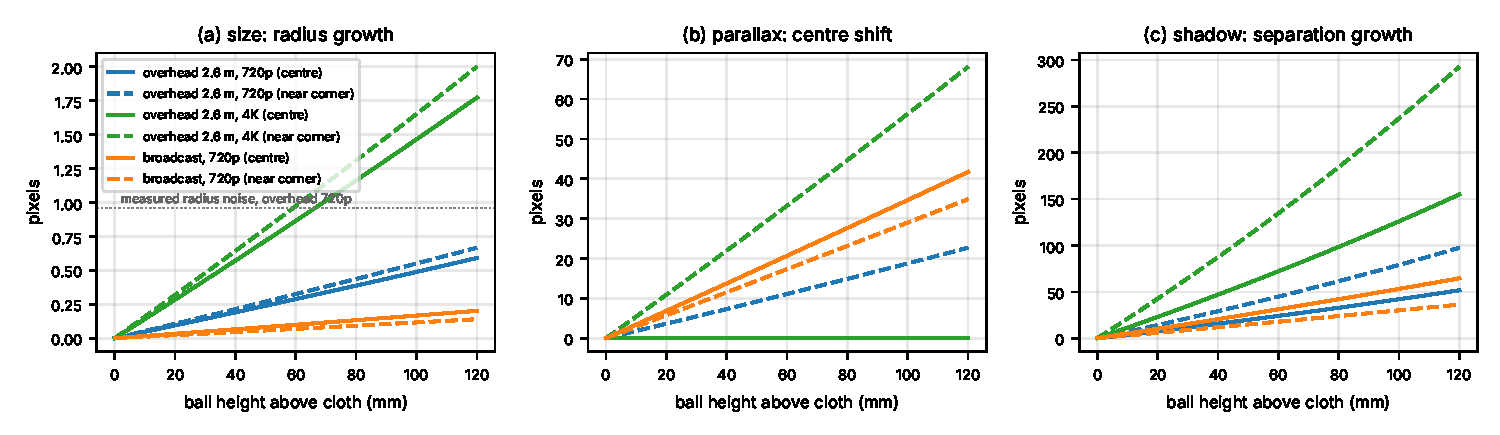
\includegraphics[width=\linewidth]{figures/cue_geometry.pdf}
\caption{Pixels of signal per cue versus ball height, for a ball at the table
centre (solid) and near a corner (dashed). Size changes are sub-pixel at any
practical resolution; overhead parallax vanishes at the nadir; lamp shadows
separate by pixels per centimetre.}
\label{fig:geometry}
\end{figure}

\section{Detector}\label{sec:detector}

The detector reads only what a deployed fixed camera has: the video, the
empty-table frame, the camera calibration (in practice from the table corners)
and the ball radius. We focus on the cue ball, which takes nearly all deliberate
jumps.

\paragraph{Tracking and measurement.}
The cue ball is found in each frame as the white connected component nearest
the predicted position. Its centre and radius are then refined using a soft
coverage mask computed against the empty-table frame. Two choices proved
essential (Sec.~\ref{sec:lessons}). First, coverage is measured as \emph{loss of
the cloth's green chromaticity} rather than as brightness above the cloth, so the
ball's unlit underside counts and shadows on the cloth do not; this cut centre
bias in the broadcast view from 2--3\,px to \TRKcentreErr\,px. Second, the
radius is taken from the coverage mask's \emph{minor} second-moment axis,
because motion blur only stretches the blob along the direction of travel.
The area-equivalent radius instead grew by up to 25\% in fast flight, and
that is a speed cue in disguise.

\paragraph{Cues.}
For each frame we compute three cue families. Each is normalised by the still
frames before the strike, which absorbs per-installation bias.
\emph{Size}: the measured radius divided by the exact silhouette radius
of an on-cloth ball at the back-projected position, with windowed mean and
maximum.
\emph{Shadow}: inside a $4.5R$ disc around the ball, pixels darker than the empty
table but with the same chromaticity are treated as shadow; we record shadow
mass, centroid offset, spread and the shadow mass just outside the ball's rim.
\emph{Motion}: on three 7-frame windows (ending at, centred on and starting at
the frame) we fit two physical models to the image track by least squares.
A \emph{rolling} model keeps the ball on the cloth, with deceleration along its
path bounded by sliding friction and a small lateral term for swerve. A
\emph{ballistic} model has free initial height and vertical velocity under
gravity, and constant horizontal velocity. The features are both residual costs, their
log ratio and the fitted height, taken from the window that most favours
flight, since a window that spans a bounce fits neither model. The ball's table
position is added as context to every cue set. We deliberately \emph{exclude}
raw speed and blur length: in any finite shot generator they correlate with
the label through the shot mix (jumps are struck hard), and a detector should
not learn that prior.

\paragraph{Classifier.}
A gradient-boosted tree classifier maps the cue vector to $P(\text{airborne})$,
smoothed with a 3-frame median; a regressor with the same features estimates the height.

\section{Experiments}\label{sec:protocol}

\paragraph{Data.}
We render \NumShots{} randomised shots (both views): half jump attempts
with first-hop apex drawn from 1.5--14\,cm and cue elevation from
25--55$^\circ$, and half level shots with random speed, spin and a slightly
elevated cue. A third of all shots place a ball on or beside the cue ball's path.
Shots in which a ball ramps off another to more than 25\,cm or leaves the table
are resampled (about 5\%). Per shot we randomise the overhead camera height
(2.2--3.0\,m), the broadcast camera placement, lamp height (0.8--1.1\,m) and
spacing (0.6--0.9\,m), sensor noise, shutter (25--100\% of the frame time) and exposure.
Shots 0--139 train and 140--199 test; the scenario clips are never trained on.

\paragraph{Labels and metrics.}
A frame is positive if the cue ball is more than 5\,mm off the cloth during the
exposure. Frames with a 1--5\,mm hop are ``don't care'' for frame metrics,
because no camera here can resolve them (Sec.~\ref{sec:geometry}). We report frame-level
average precision (AP), event recall, where an event is a flight with apex
$>$5\,mm, bounces are merged, and the event counts as detected if at least two of its frames fire, and false alarms per minute of video,
i.e.\ predicted runs of at least two frames that touch no airborne frame. Thresholds are chosen
by grouped 5-fold cross-validation on the training shots only.

\section{Results}\label{sec:results}

\begin{table}[t]
\centering\small
\begin{tabular}{lrrrrrrrrr}
\toprule
 & \multicolumn{3}{c}{Overhead} & \multicolumn{3}{c}{Broadcast} & \multicolumn{3}{c}{Both views} \\
\cmidrule(lr){2-4}\cmidrule(lr){5-7}\cmidrule(lr){8-10}
Cues & AP & Ev.\,rec. & FA/min & AP & Ev.\,rec. & FA/min & AP & Ev.\,rec. & FA/min \\
\midrule
size & 0.62 & 0.74 & 20.9 & 0.40 & 0.64 & 20.4 & 0.71 & 0.69 & 11.2 \\
shadow & 0.78 & 0.87 & 6.8 & 0.79 & 0.87 & 14.1 & 0.87 & 0.92 & 11.2 \\
motion & 0.59 & 1.00 & 24.3 & 0.86 & 0.77 & 8.3 & 0.91 & 0.87 & 11.2 \\
size+shadow & 0.81 & 0.90 & 15.6 & 0.79 & 0.87 & 11.2 & 0.87 & 0.85 & 8.3 \\
size+motion & 0.73 & 0.74 & 11.2 & 0.90 & 0.82 & 4.4 & 0.95 & 0.87 & 6.8 \\
shadow+motion & 0.85 & 0.92 & 13.6 & 0.92 & 0.85 & 9.2 & 0.96 & 0.90 & 5.8 \\
all & 0.86 & 0.82 & 12.6 & 0.93 & 0.79 & 3.4 & 0.96 & 0.90 & 4.9 \\
\midrule
Height MAE (mm) & \multicolumn{3}{c}{14} & \multicolumn{3}{c}{14} & \multicolumn{3}{c}{11} \\
\bottomrule
\end{tabular}

\caption{Cue ablation on \NumTest{} held-out shots (\NumEvents{} jump events).
AP: frame-level average precision. Ev.\,rec.: event recall. FA/min: false alarms per minute
of video. Last row: mean absolute error of the regressed height on airborne frames.}
\label{tab:ablation}
\end{table}

\INPUTRESULTTEXT

\begin{figure}[t]
\centering
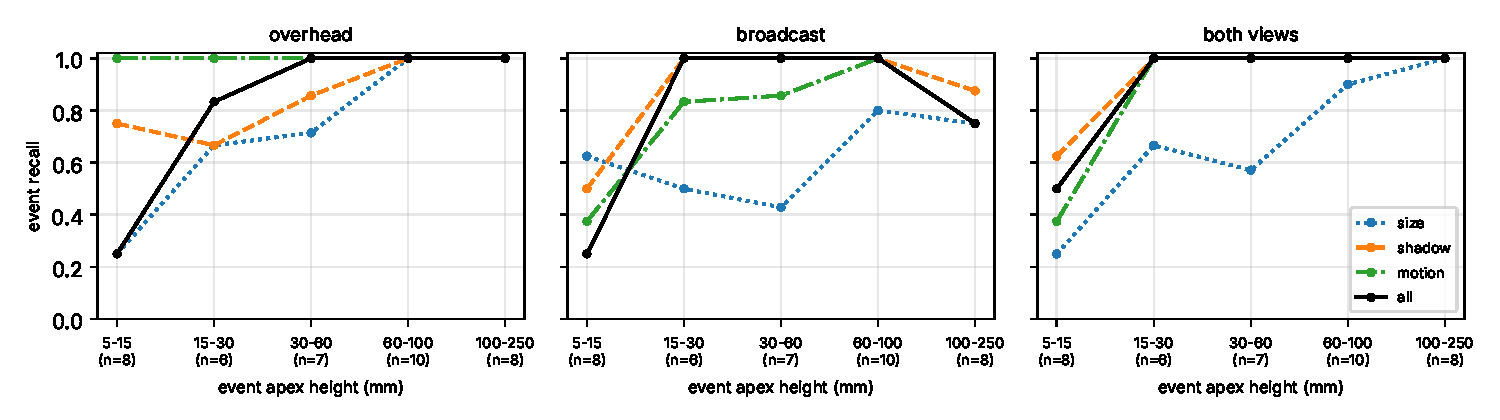
\includegraphics[width=\linewidth]{figures/recall_vs_apex.pdf}
\caption{Event recall versus the apex height of the flight, per cue family and camera.}
\label{fig:apex}
\end{figure}

\begin{figure}[t]
\centering
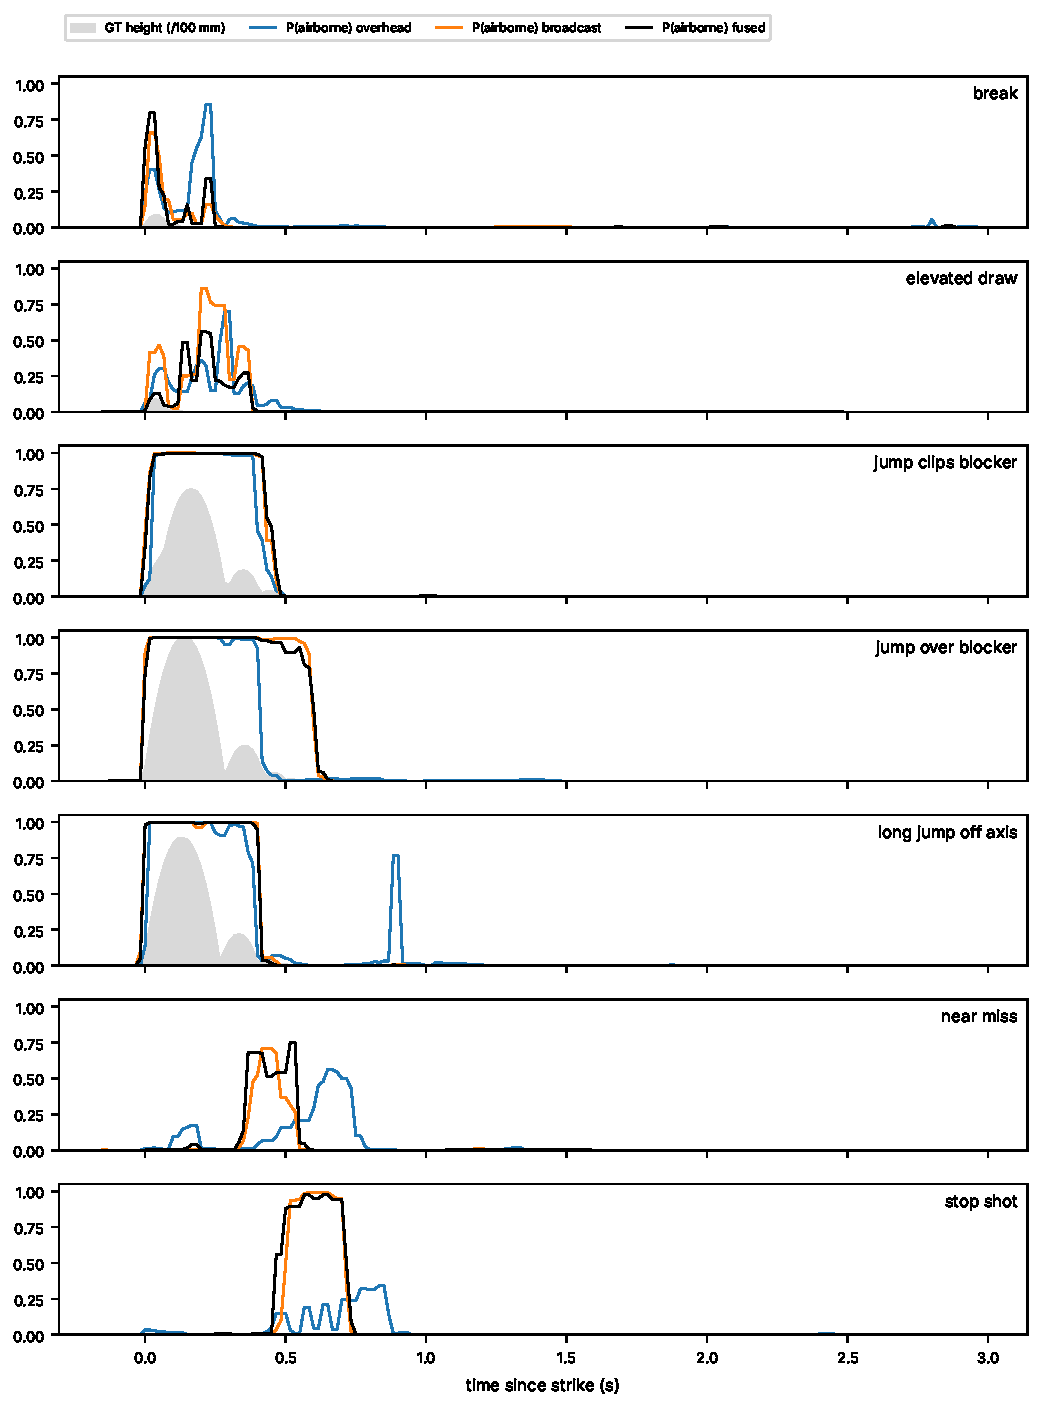
\includegraphics[width=0.85\linewidth]{figures/showcase_timeseries.pdf}
\caption{Scenario clips: predicted $P(\text{airborne})$ of the all-cue detectors
(trained on random shots only) against the ground-truth cue-ball height (grey).}
\label{fig:showcase}
\end{figure}

\section{Lessons from building the detector}\label{sec:lessons}
Three failure modes appeared before any learning, and all three would also
afflict real footage. (i) \emph{Brightness-based segmentation} misses the
unlit underside of the ball in the broadcast view; the resulting radius
estimate drifted by 15\% as the ball moved under different lamps, far more
than the 4--7\% that 10\,cm of height produces. (ii) \emph{Motion blur
inflates area}: a fast airborne cue ball looked 10--25\% larger from
overhead, while the true geometric change was 2--4\%. A size cue measured by
area is mostly a speed cue. (iii) \emph{Unconstrained motion models explain
flight}: a rolling model with free 2D acceleration fits the apparent ground
track of a short flight about as well as a ballistic model. The model
comparison only becomes informative once rolling deceleration is bounded by
friction.

\section{Towards real clips}\label{sec:real}

The synthetic study fixes what to measure; the open question is transfer. We
propose collecting real clips with height ground truth instead of scraping
broadcast footage, which has none. A phone fixed overhead at about 2.5\,m
serves as the overhead view, a second camera behind the foot rail as the
broadcast view, and a third camera at cloth level, perpendicular to the shot
line, records 240\,fps slow motion. That third view gives the ball's height
directly against a printed scale on the rail, and a clap or LED flash
synchronises the cameras. The shot list mirrors Table~\ref{tab:clips}: jumps over
blockers at several distances, jumps that clip the blocker, near-misses,
elevated draw and follow shots, breaks, and level shots at all speeds. The
protocol, labelling scheme and a clip checklist are in
\texttt{data/real/README.md}.

\section{Limitations}
The ground truth is exact only for the simulated world. The physics omits
cloth compression, ball--ball friction (throw) and the cue--ball--slate
interaction during a jump, and $e_t$ is a single constant. The renderer has
no reflections, cloth texture, people or occlusion by players and cues, which a
real overhead feed will contain. We detect the cue ball only; object-ball
hops (present in two scenario clips) are left for future work. Most
importantly, nothing here has been validated on real video yet.

\section{Conclusion}
\INPUTRESULTCONCLUSION

\bibliographystyle{plainnat}
\bibliography{refs}
\end{document}
